% interactcadsample.tex
% v1.03 - April 2017

\documentclass[]{interact}

\usepackage{epstopdf}% To incorporate .eps illustrations using PDFLaTeX, etc.
\usepackage{subfigure}% Support for small, `sub' figures and tables
%\usepackage[nolists,tablesfirst]{endfloat}% To `separate' figures and tables from text if required

\usepackage{natbib}% Citation support using natbib.sty
\bibpunct[, ]{(}{)}{;}{a}{}{,}% Citation support using natbib.sty
\renewcommand\bibfont{\fontsize{10}{12}\selectfont}% Bibliography support using natbib.sty

\theoremstyle{plain}% Theorem-like structures provided by amsthm.sty
\newtheorem{theorem}{Theorem}[section]
\newtheorem{lemma}[theorem]{Lemma}
\newtheorem{corollary}[theorem]{Corollary}
\newtheorem{proposition}[theorem]{Proposition}

\theoremstyle{definition}
\newtheorem{definition}[theorem]{Definition}
\newtheorem{example}[theorem]{Example}

\theoremstyle{remark}
\newtheorem{remark}{Remark}
\newtheorem{notation}{Notation}


% tightlist command for lists without linebreak
\providecommand{\tightlist}{%
  \setlength{\itemsep}{0pt}\setlength{\parskip}{0pt}}



\usepackage{hyperref}
\usepackage[utf8]{inputenc}
\def\tightlist{}
\usepackage{setspace}


\begin{document}


\articletype{Short Technical Note}

\title{A new simplified manual tour, with examples in mathematica}


\author{\name{Alex Aumann$^{a}$, German Valencia$^{a}$, Ursula
Laa$^{b}$, Dianne Cook$^{c}$}
\affil{$^{a}$School of Physics and Astronomy, Monash
University; $^{b}$Institute of Statistics, University of Natural
Resources and Life Sciences, Vienna; $^{b}$Department of Econometrics
and Business Statistics, Monash University}
}

\thanks{CONTACT Alex
Aumann. Email: \href{mailto:aaum0002@student.monash.edu}{\nolinkurl{aaum0002@student.monash.edu}}, German
Valencia. Email: \href{mailto:german.valencia@monash.edu}{\nolinkurl{german.valencia@monash.edu}}, Ursula
Laa. Email: \href{mailto:ursula.laa@boku.ac.at}{\nolinkurl{ursula.laa@boku.ac.at}}, Dianne
Cook. Email: \href{mailto:dicook@monash.edu}{\nolinkurl{dicook@monash.edu}}}

\maketitle

\begin{abstract}
Something here
\end{abstract}

\begin{keywords}
data visualisation; grand tour; statistical computing; statistical
graphics; multivariate data; dynamic graphics
\end{keywords}

\%\doublespacing \# Introduction

\hypertarget{sec:method}{%
\section{Manual tour}\label{sec:method}}

\begin{figure}
\centering
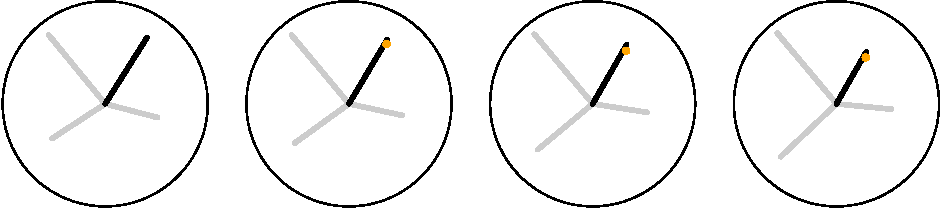
\includegraphics{paper_files/figure-latex/manualsequence-1.pdf}
\caption{Sequence of projections where V3 contribution is changed.}
\end{figure}

\hypertarget{background}{%
\subsection{Background}\label{background}}

\hypertarget{new-definition}{%
\subsection{New definition}\label{new-definition}}

\hypertarget{sec:implementation}{%
\section{Implementation}\label{sec:implementation}}

\hypertarget{sec:examples}{%
\section{Applications}\label{sec:examples}}

\hypertarget{sec:discussion}{%
\section{Discussion}\label{sec:discussion}}

\hypertarget{acknowledgements}{%
\section*{Acknowledgements}\label{acknowledgements}}
\addcontentsline{toc}{section}{Acknowledgements}

The authors gratefully acknowledge the support of the Australian
Research Council. The paper was written in \texttt{rmarkdown}
\citep{rmarkdown} using \texttt{knitr} \citep{knitr}.

\hypertarget{supplementary-material}{%
\section*{Supplementary material}\label{supplementary-material}}
\addcontentsline{toc}{section}{Supplementary material}

The source material and animated gifs for this paper are available at

\bibliographystyle{tfcad}
\bibliography{biblio.bib}





\end{document}
